% !TeX root = ../../../book.tex
\subsection{示例和伪例}

``语法正确''是指句子中的单词和符号被正确组合且具有明确含义。这排除了无意义的符号或单词组合,例如:
\begin{center}
    \textcolor{red}{$1+ = 2$, $\text{Fisher}^2 = 1$, $\big\{\{\varnothing\}\big\} - 7 > 5\pi$, $\text{You am smart}$}
\end{center}
以上第三个例子并非数学陈述,因为 $\big\{\{\varnothing\}\big\}$ 不是数字,无法解释如何从该集合中``减去 $7$''。

而``\emph{唯一}真值''要求陈述要么为\verb|真|要么为\verb|假|,不能同时成立,也不能非真非假。这排除了``\textcolor{red}{$x^2 - 1 = 0$}''这类陈述——若未声明 $x$ 的取值,则无法判定其真值。

\subsubsection*{真值未知}

定义中的有趣之处在于:即使能确定真值唯一,我们仍可能不知其具体结果。例如:
\begin{center}
    \textcolor{olivegreen}{任何大于或等于 $4$ 的偶自然数均可表示为两个质数之和。}
\end{center}

此命题是真是假?若能证明或证伪,数学界将为之振奋!该命题称为\href{https://baike.baidu.com/item/哥德巴赫猜想/72364}{哥德巴赫猜想}\footnote{术语说明:\textbf{猜想}指被认为成立但尚未被证明或证伪的命题。},是数学中著名的未解难题(我们相信只是暂时的!)。尽管目前无人知晓其真伪,可以肯定的是,\emph{仅有一个}真值适用:该命题不可能既\verb|真|又\verb|假|,也不可能存在中间状态。要么所有不小于 $4$ 的偶自然数都具有此性质,要么存在反例。即使尚未知晓正确答案,这种``非此即彼''的特性仍然成立。因此该命题完全满足\emph{数学陈述}的定义。

\subsubsection*{悖论语句}

使陈述没有真值的一种方法是构造\textbf{悖论}。考虑以下陈述:
\begin{center}
    \textcolor{red}{这句话是假的。}
\end{center}
这显得十分怪异,因为该语句直接断言了自身的真值。现在分析其可能的真值:
\begin{itemize}
    \item 假设这句话为\verb|真|。那么,根据其内容,它实际上为\verb|假|。
    \item 假设这句话为\verb|假|。同理,根据其内容,它实际上为\verb|真|。
\end{itemize}
这种矛盾无法调和!这句话某种程度上同时具有\verb|真|与\verb|假|的双重属性,或处于某种非真非假的状态。由于数学体系需要避免此类异常现象,我们的定义将明确排除这类语句。

(\emph{思考题}:若允许此类语句作为合法数学陈述,会产生什么后果?若放弃``每句话必为\verb|真|或为\verb|假|''的基本原则,数学体系是否仍能自洽?这会引发矛盾,还是创造出一个全新的数学宇宙?)

通常,这种\textbf{自指}语句(即指向自身的陈述)极易引发悖论,这正是我们需要禁止的。

\begin{multicols}{2}
    该悖论的变体可以通过右侧这幅卡通漫画说明:当皮诺曹说``我的鼻子要变长''时会发生什么?若此言为真,则鼻子会伸长——但皮诺曹的鼻子仅在说谎时才会变长。若此言为假,则鼻子会伸长(符合说谎特征),而这反而验证了陈述的真实性!如此形成无法解开的逻辑循环。

    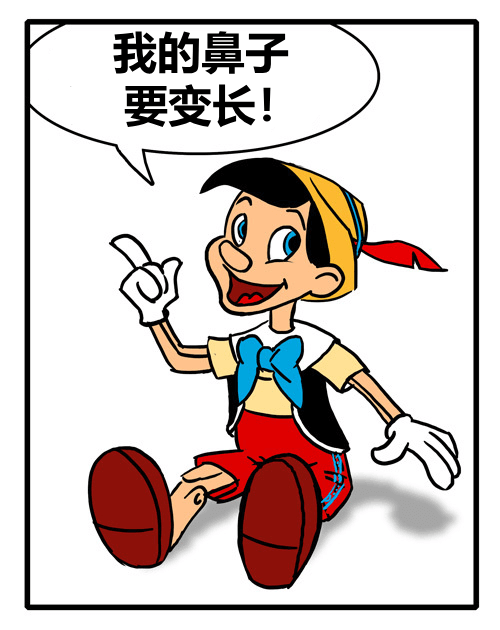
\includegraphics[scale=0.3]{figure/pinocchio.png}
\end{multicols}

更复杂的案例是\emph{奎因悖论 (Quine's Paradox)}:
\begin{center}
    \textcolor{red}{``Yields falsehood when preceded by its quotation'' \\yields falsehood when preceded by its quotation.}
\end{center}
此悖论留待读者自行探索。此类自相矛盾的陈述具有本质上的病态特征,因此我们的定义将直接排除它们。
